\documentclass[preprint,
3p]{elsarticle} %review=doublespace preprint=single 5p=2 column
%%% Begin My package additions %%%%%%%%%%%%%%%%%%%

\usepackage[hyphens]{url}

  \journal{Remote Sensing of Environment} % Sets Journal name

\usepackage{graphicx}
%%%%%%%%%%%%%%%% end my additions to header

\usepackage[T1]{fontenc}
\usepackage{lmodern}
\usepackage{amssymb,amsmath}
% TODO: Currently lineno needs to be loaded after amsmath because of conflict
% https://github.com/latex-lineno/lineno/issues/5
\usepackage{lineno} % add
\usepackage{ifxetex,ifluatex}
\usepackage{fixltx2e} % provides \textsubscript
% use upquote if available, for straight quotes in verbatim environments
\IfFileExists{upquote.sty}{\usepackage{upquote}}{}
\ifnum 0\ifxetex 1\fi\ifluatex 1\fi=0 % if pdftex
  \usepackage[utf8]{inputenc}
\else % if luatex or xelatex
  \usepackage{fontspec}
  \ifxetex
    \usepackage{xltxtra,xunicode}
  \fi
  \defaultfontfeatures{Mapping=tex-text,Scale=MatchLowercase}
  \newcommand{\euro}{€}
\fi
% use microtype if available
\IfFileExists{microtype.sty}{\usepackage{microtype}}{}
\usepackage[]{natbib}
\bibliographystyle{apalike}

\ifxetex
  \usepackage[setpagesize=false, % page size defined by xetex
              unicode=false, % unicode breaks when used with xetex
              xetex]{hyperref}
\else
  \usepackage[unicode=true]{hyperref}
\fi
\hypersetup{breaklinks=true,
            bookmarks=true,
            pdfauthor={},
            pdftitle={Comprehensive assessment of the climate-induced water scarcity over continental Chile},
            colorlinks=false,
            urlcolor=blue,
            linkcolor=magenta,
            pdfborder={0 0 0}}

\setcounter{secnumdepth}{5}
% Pandoc toggle for numbering sections (defaults to be off)


% tightlist command for lists without linebreak
\providecommand{\tightlist}{%
  \setlength{\itemsep}{0pt}\setlength{\parskip}{0pt}}




\usepackage{booktabs}
\usepackage{longtable}
\usepackage{array}
\usepackage{multirow}
\usepackage{wrapfig}
\usepackage{float}
\usepackage{colortbl}
\usepackage{pdflscape}
\usepackage{tabu}
\usepackage{threeparttable}
\usepackage{threeparttablex}
\usepackage[normalem]{ulem}
\usepackage{makecell}
\usepackage{xcolor}



\begin{document}


\begin{frontmatter}

  \title{Comprehensive assessment of the climate-induced water scarcity
over continental Chile}
    \author[Hemera Centro de Observación de la Tierra,Universidad
Mayor]{Francisco Zambrano%
  \corref{cor1}%
  \fnref{1}}
   \ead{francisco.zambrano@umayor.com} 
    \author[Another University]{Bob Security%
  %
  }
   \ead{bob@example.com} 
    \author[Another University]{Cat Memes%
  %
  \fnref{2}}
   \ead{cat@example.com} 
    \author[Some Institute of Technology]{Derek Zoolander%
  %
  \fnref{2}}
   \ead{derek@example.com} 
      \affiliation[Hemera Centro de Observación de la Tierra]{
    organization={Facultad de Ciencias, Universidad
Mayor.},addressline={La Piramide
5750},city={Santiago},postcode={123456},state={Huechuraba},country={United
States},}
    \affiliation[Another University]{
    organization={Department},addressline={A street
29},city={Manchester,},postcode={2054 NX},country={The Netherlands},}
    \cortext[cor1]{Corresponding author}
    \fntext[1]{This is the first author footnote.}
    \fntext[2]{Another author footnote.}
  
  \begin{abstract}
  Human-induced greenhouse gas emissions have increased the frequency
  and/or intensity of some weather and climate extremes globally. Chile
  has been affected by persistent water scarcity which has been
  impacting the hydrological system and vegetation development. Central
  Chile it is been the focus of research studies due to the diminishing
  of water supply, nevertheless water deficit is expanded beyond,
  specifically to the south of the country.
  \end{abstract}
    \begin{keyword}
    keyword1 \sep 
    keyword2
  \end{keyword}
  
 \end{frontmatter}

\hypertarget{version}{%
\section{Version}\label{version}}

This Rmd-skeleton uses the mdpi Latex template published 2019/02.
However, the official template gets more frequently updated than the
`rticles' package. Therefore, please make sure prior to paper
submission, that you're using the most recent .cls, .tex and .bst files
(available \href{http://www.mdpi.com/authors/latex}{here}).

\hypertarget{introduction}{%
\section{Introduction}\label{introduction}}

The sixth assessment report (AR6) from the working group I of the IPCC
\citep{IPCC2021} indicates that human-induced greenhouse gas emissions
have increased the frequency and/or intensity of some weather and
climate extremes and the evidence has been strengthened since AR5
\citep{IPCC2013}. There is high confidence that the increasing global
warning can expand the land area affected by increasing drought
frequency and severity \citep{IPCCCH112021}. Chile has been facing a
persistent rainfall deficit lasting for more than ten years
\citep{Garreaud2017} which has impacted the hydrological system
\citep{Boisier2018}, and consequently the vegetation development
\citep{Zambrano2020}.

Precipitation is the primary driver of drought that impacts hydrological
regimes and vegetation productivity. Thus, it is commonly classified as
meteorological, hydrological, and agricultural \citep{Wilhite1985}.
Lately, it has been argued that this definition does not fully address
the ecological dimensions \citep{Crausbay2017}. \citet{Crausbay2017}
proposed the ecological drought definition as ``an episodic deficit in
water availability that drives ecosystems beyond thresholds of
vulnerability, impacts ecosystem services, and triggers feedback in
natural and/or human systems''. The AR6 \citep{IPCC2021} state that even
if global warming is stabilized at 1.5°-2°C many parts of the world will
be impacted by more severe agricultural and ecological drought. Central
Chile has suffered from crop productivity failure, highlighting the
growing season 2007-2008 and 2008-2009
\citep{Zambrano2016, Zambrano2018}, which impacted an extensive surface.
But, in 2019-2020, the drought intensity reached an extreme condition at
North 34°S not seen -at least- for more than 40 years
\citep{Zambrano2020}, affecting forest, grassland, and croplands areas.
The prolonged lack of precipitation within Central Chile is producing
changes in the ecosystem that should study.

Satellite remote sensing \citep{West2019, AghaKouchak2015} is the
primary method to evaluate how meteorological drought impacts vegetation
dynamics. Since the 90's multiple vegetation drought indices have been
derived (VCI,\citep{Kogan1990}; TCI, \citep{Kogan1995};zNDVI,
\citep{Peters2002}; VegDri, \citep{Brown2008}) that have allowed making
spatiotemporal analysis. Although we can calculate those indices for any
time during the year (depending on satellite revisit), there are
relevant during the stage vegetation has more activity, the growing
season \citep{Mishra2015}. Although modeling phenology is a complex
task, satellites offer strategies that help to address it
\citep{Younes2021, Vrieling2018, Cai2017}. Also, the land cover dynamics
product MCD12Q2 from the USGS \citep{Friedl2019} provides some phenology
metrics. Some authors have proposed indices aggregated during the
season. \citet{Meroni2017} accumulating the fractional active
photosynthetic active radiation(FAPAR) between the start (SOS) and the
end of the season (EOS) in the Sahel, calculate the zCFAPAR.
\citet{Zambrano2018} used the same approach but with the NDVI
(Normalized Difference Vegetation Index), derivating the zcNDVI within
Central Chile. Besides, land use land cover (LULC) change can be driven
by drought \citep{Tran2019, Akinyemi2021}. To analyze those changes,
multiple time-series LULC products exist as the MCD12Q1
\citep{Friedl2019} and the ESA CCI-LC \citep{ESA2017}. For Chile, 2014
was made a high-resolution land cover at 30m of spatial resolution
\citep{Zhao2016}. The LULC product with the vegetation drought index can
help evaluate the impact of drought on the ecosystem.

Vegetation drought indices are commonly used as proxies of productivity
\citep{Paruelo2016, Schucknecht2017}. The main environmental variables
that affect productivity are water supply and demand \citep{Mishra2015}.
Those are measured by precipitation and evapotranspiration (ET),
commonly collected from weather stations. Usually, in developing
countries (i.e., Chile), incomplete records or gaps present a challenge.
But, there are satellite estimates of these variables. To evaluate
drought, the World Meteorological Organization (WMO; \citep{WMO2012})
has proposed the Standardized Precipitation Index (SPI;
\citep{McKee1993}), a multiscalar drought index, which has been used
worldwide. For Chile, \citet{Zambrano2017} derived and evaluated it from
the product of the Climate Hazards Group InfraRed Precipitation with
Station data (CHIRPS; \citep{Funk2015}). For water demand, it is used
ET. The vegetation biomass productivity is strongly related to ET
\citep{FAO66}. The atmospheric evaporative demand (AED) represents the
maximum ET rate from a land surface (without water restriction), also
known as reference ET. The recommended method for its calculation is the
FAO Penman-Monteith \citep{Pereira2015, Allen2005}. Due to climate
change, AED is increasing, driving ET rise \citep{IPCCCH112021}. But, it
is not always true \citep{Milly2016}. For example, regions where AET is
highest have the lowest ET. The MOD16 product
\citep{Running2021, Mu2011} provides AET and ET satellite estimates and
has been used to derive drought indices \citep{Mu2013}. Soil moisture
(SM) is an Essential Climate Variable (ECV) that modulates vegetative
growth. The climate change initiative (CCI) from the European Space
Agency (ESA) delivers the ESA CCI SM product \citep{Dorigo2017} (current
version 6.1), which has been helpful to monitor drought
\citep{Zhang2019}. Besides, total water storage can be retrieved by the
Gravity Recovery and Climate Experiment (GRACE), which allows analyzing
water availability changes \citep{Ahmed2014, Ma2017}. The water demand
and supply by remote sensing can help evaluate how they have impacted
vegetation productivity.

We aims to analyze the climate-induced water scarcity over continental
Chile for 2000-2023 by using estimated environmental variables of
biomass productivity, and water demand/supply gather from earth
observation products. The specific objective for the study are i) to
evaluate LULC change for 2001-2021, ii) to derive and assess the
vegetation drought index zcNDVI as a proxy of biomass productivity, iii)
analyze the interconnection of zcNDVI with drought indices of supply
(i.e., precipitation), demand (i.e, ET), and vegetation cover; and iv)
we will investigate if the observed changes are linked to the TWS and
SM.

\hypertarget{study-area}{%
\section{Study area}\label{study-area}}

\begin{figure}[!ht]
\centering
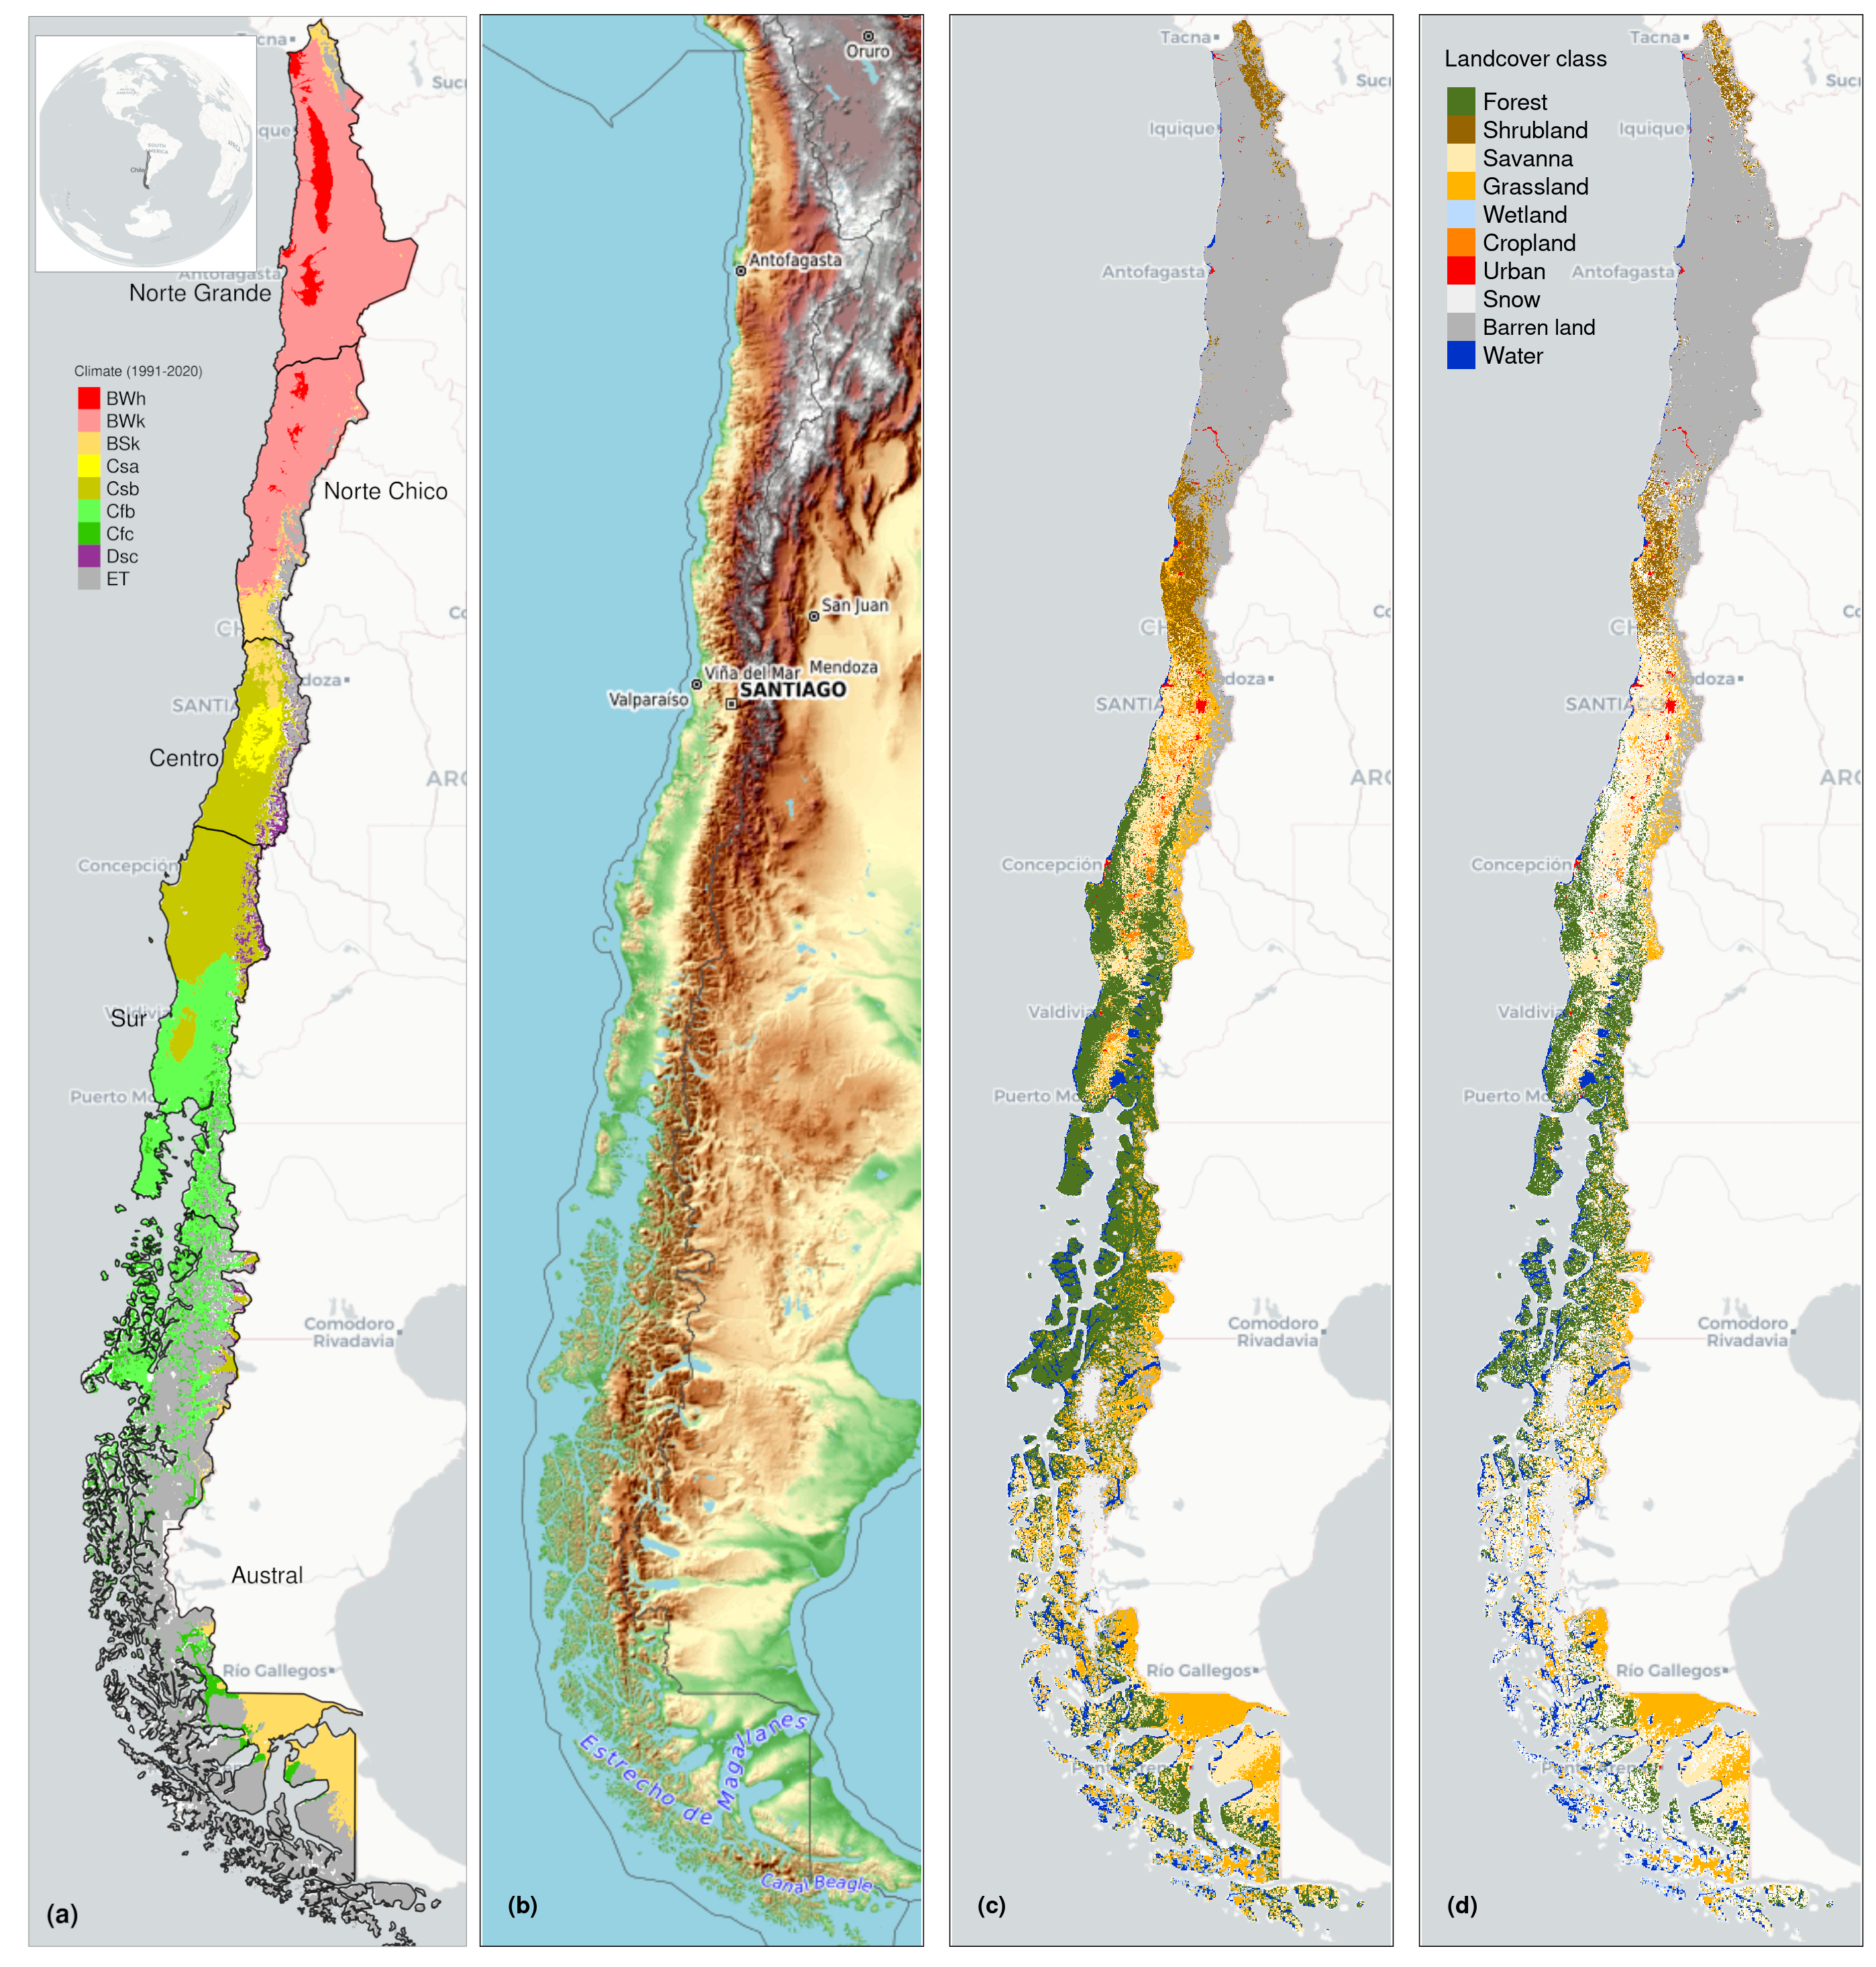
\includegraphics[width=\textwidth]{../output/figs/map_study_con_landcover.png}
\caption{ (\textbf{a}) Location of Central Chile and zones north (NCCH), central (CCCH), and south (SCCH) Central Chile. (\textbf{b}) Topography reference map. (\textbf{c}) Land cover classes for 2019. (\textbf{d}) Persistent land cover classess (> 80\%) for 2001-2021.}
\end{figure}

\hypertarget{materials-and-methods}{%
\section{Materials and Methods}\label{materials-and-methods}}

\hypertarget{data}{%
\subsection{Data}\label{data}}

\hypertarget{satellite-data}{%
\subsubsection{Satellite data}\label{satellite-data}}

\hypertarget{in-situ-data}{%
\subsubsection{in-situ data}\label{in-situ-data}}

\hypertarget{lulc-change-for-2001-2021}{%
\subsection{LULC change for 2001-2021}\label{lulc-change-for-2001-2021}}

\hypertarget{landcover-change-and-persistence}{%
\subsubsection{Landcover change and
persistence}\label{landcover-change-and-persistence}}

\hypertarget{drought-index-for-biomass-productivity-zcndvi}{%
\subsection{Drought index for biomass productivity
zcNDVI}\label{drought-index-for-biomass-productivity-zcndvi}}

\hypertarget{interconnection-of-productivity-with-drought-indices-of-supplydemand-and-vegetation-cover}{%
\subsection{Interconnection of productivity with drought indices of
supply/demand and vegetation
cover}\label{interconnection-of-productivity-with-drought-indices-of-supplydemand-and-vegetation-cover}}

\hypertarget{totatl-water-storage-and-soil-moisture}{%
\subsection{Totatl water storage and Soil
Moisture}\label{totatl-water-storage-and-soil-moisture}}

\hypertarget{results}{%
\section{Results}\label{results}}

\hypertarget{lulc-change-for-2001-2021-1}{%
\subsection{LULC change for
2001-2021}\label{lulc-change-for-2001-2021-1}}

\begin{table}[!ht]

\caption{\label{tab:unnamed-chunk-1}Value of linear change trend next to time-series plot of surface, per landcover class (IGBP MCD12Q1.006) for 2001-2019 through Central Chile. Red dots on the plots indicate the maximum and minimum surface.}
\centering
\resizebox{\linewidth}{!}{
\begin{tabular}[t]{r>{}r>{}r>{}r>{}r>{}r>{}r}
\toprule
\multicolumn{1}{c}{ } & \multicolumn{6}{c}{Trend of change [$km^2 year^{-1}$]} \\
\cmidrule(l{3pt}r{3pt}){2-7}
zone & Shrubland & Savanna & Grassland & Barren land & Forest & Cropland\\
\midrule
norte grande & -2.3
\includegraphics[width=0.67in, height=0.17in]{article_files/figure-latex//plot_19671073045199.pdf} & 0.1
\includegraphics[width=0.67in, height=0.17in]{article_files/figure-latex//plot_19671013721869.pdf} & -31.2
\includegraphics[width=0.67in, height=0.17in]{article_files/figure-latex//plot_19671079e41f67.pdf} & 32.8
\includegraphics[width=0.67in, height=0.17in]{article_files/figure-latex//plot_19671075ebd9d8.pdf} & NA
\includegraphics[width=0.67in, height=0.17in]{article_files/figure-latex//plot_196710524640a1.pdf} & NA
\includegraphics[width=0.67in, height=0.17in]{article_files/figure-latex//plot_19671012073e8a.pdf}\\
norte chico & 79.3
\includegraphics[width=0.67in, height=0.17in]{article_files/figure-latex//plot_19671061580771.pdf} & -66.1
\includegraphics[width=0.67in, height=0.17in]{article_files/figure-latex//plot_1967101832bef9.pdf} & -100.2
\includegraphics[width=0.67in, height=0.17in]{article_files/figure-latex//plot_1967105771ba87.pdf} & 104.0
\includegraphics[width=0.67in, height=0.17in]{article_files/figure-latex//plot_19671042ea518f.pdf} & 0.0
\includegraphics[width=0.67in, height=0.17in]{article_files/figure-latex//plot_196710607baab3.pdf} & -13.1
\includegraphics[width=0.67in, height=0.17in]{article_files/figure-latex//plot_1967106f91099.pdf}\\
zona central & 130.2
\includegraphics[width=0.67in, height=0.17in]{article_files/figure-latex//plot_1967105c411aeb.pdf} & -128.6
\includegraphics[width=0.67in, height=0.17in]{article_files/figure-latex//plot_1967108a6119a.pdf} & 89.9
\includegraphics[width=0.67in, height=0.17in]{article_files/figure-latex//plot_19671016b408b2.pdf} & 23.3
\includegraphics[width=0.67in, height=0.17in]{article_files/figure-latex//plot_1967103ee6f936.pdf} & -66.2
\includegraphics[width=0.67in, height=0.17in]{article_files/figure-latex//plot_19671074c30c6.pdf} & -24.4
\includegraphics[width=0.67in, height=0.17in]{article_files/figure-latex//plot_19671056667823.pdf}\\
zona sur & -14.6
\includegraphics[width=0.67in, height=0.17in]{article_files/figure-latex//plot_1967106cc832ad.pdf} & -316.2
\includegraphics[width=0.67in, height=0.17in]{article_files/figure-latex//plot_19671034e3692f.pdf} & -55.9
\includegraphics[width=0.67in, height=0.17in]{article_files/figure-latex//plot_1967104ac90971.pdf} & 2.1
\includegraphics[width=0.67in, height=0.17in]{article_files/figure-latex//plot_1967107f7df47e.pdf} & 412.4
\includegraphics[width=0.67in, height=0.17in]{article_files/figure-latex//plot_1967104e385249.pdf} & 30.8
\includegraphics[width=0.67in, height=0.17in]{article_files/figure-latex//plot_19671013698bfb.pdf}\\
zona austral & -44.6
\includegraphics[width=0.67in, height=0.17in]{article_files/figure-latex//plot_196710491ed82a.pdf} & 163.9
\includegraphics[width=0.67in, height=0.17in]{article_files/figure-latex//plot_196710190c87cf.pdf} & 226.1
\includegraphics[width=0.67in, height=0.17in]{article_files/figure-latex//plot_1967101d6ab929.pdf} & -80.2
\includegraphics[width=0.67in, height=0.17in]{article_files/figure-latex//plot_19671033cd1ca4.pdf} & -9.1
\includegraphics[width=0.67in, height=0.17in]{article_files/figure-latex//plot_1967101f22c71d.pdf} & -1.0
\includegraphics[width=0.67in, height=0.17in]{article_files/figure-latex//plot_196710336ead1.pdf}\\
\bottomrule
\end{tabular}}
\end{table}

\hypertarget{landcover-change-and-persistence-1}{%
\subsubsection{Landcover change and
persistence}\label{landcover-change-and-persistence-1}}

\hypertarget{drought-index-for-biomass-productivity-zcndvi-1}{%
\subsection{Drought index for biomass productivity
zcNDVI}\label{drought-index-for-biomass-productivity-zcndvi-1}}

\hypertarget{interconnection-of-productivity-with-drought-indices-of-supplydemand-and-vegetation-cover-1}{%
\subsection{Interconnection of productivity with drought indices of
supply/demand and vegetation
cover}\label{interconnection-of-productivity-with-drought-indices-of-supplydemand-and-vegetation-cover-1}}

\hypertarget{total-water-storage-and-soil-moisture}{%
\subsection{Total water storage and Soil
Moisture}\label{total-water-storage-and-soil-moisture}}

\begin{figure}[!ht]
\centering
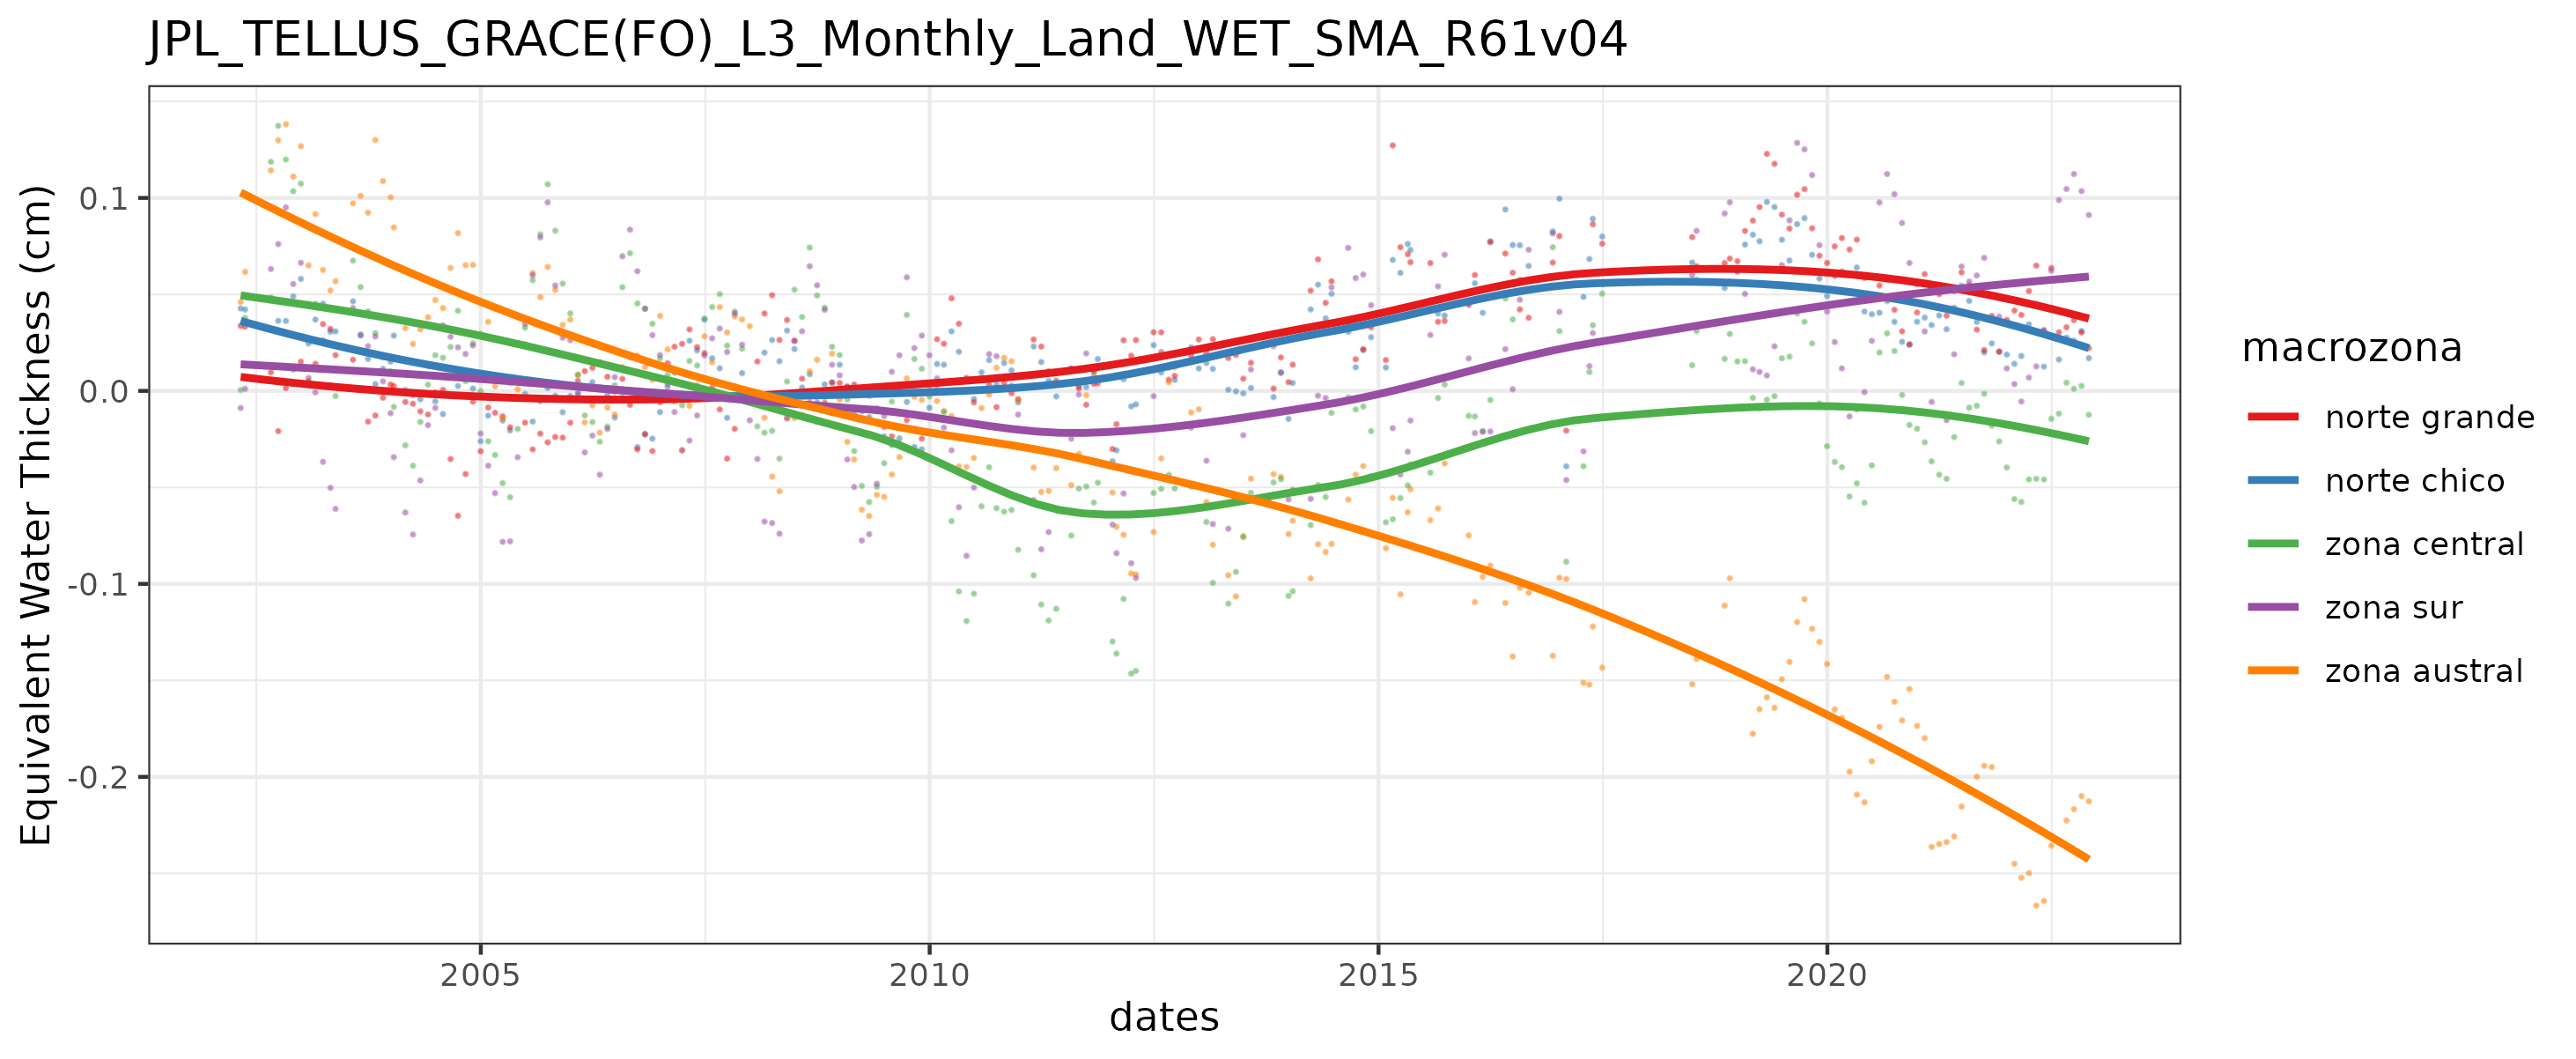
\includegraphics[width=\textwidth]{../output/figs/JPL_TELLUS_GRACE-FO_L3_Monthly_Land_WET_SMA_R61v04_macrozonas.png}
\caption{Total water storage (mm) trend for 2002-2023 in the five macrozones on continental Chile}
\end{figure}

\hypertarget{discussion}{%
\section{Discussion}\label{discussion}}

Authors should discuss the results and how they can be interpreted in
perspective of previous studies and of the working hypotheses. The
findings and their implications should be discussed in the broadest
context possible. Future research directions may also be highlighted.

\hypertarget{conclusion}{%
\section{Conclusion}\label{conclusion}}

This section is not mandatory, but can be added to the manuscript if the
discussion is unusually long or complex.

\renewcommand\refname{References}
\bibliography{references.bib}


\end{document}
